\chapter{Air Traffic monitoring: a use case}

\section{Introduction}

Air traffic monitoring can be considered a practical use case for the infrastructure described in the previous chapters, being characterised by the Big Data 3 Vs, as there are more than 5000 aircrafts flying any time (Volume), each one of which is transmitting data via transponder signals once every few seconds (Velocity) and, for each data source, data formats can be wildly different from one another, while, additionally, raw data transmitted by aircrafts can be used in conjunction with other kinds of data, such as weather and social networks, for deeper analytics (Variety).

\section{Infrastructure overview}

The infrastructure bones have been built with a series of Virtual Machines provisioned in the Azure Pack Cloud-On-Premise environment provided by the VarGroup Data Center located in Empoli (FI). There are, in total, seven VMs mounting CentOS 7 and the following specifications:
\\
% Table with specifications
\\
All of these VMs are part of an \textbf{Hortonworks} cluster featuring HDP 2.6.1, deployed via Ambari Blueprint interface through an aptly made scripting suite to automate machine preparation. As additional software used, other than Hortonworks Hadoop distribution, which includes HDFS, YARN, Spark 2, Hive, Kafka, Zookeeper, Ranger, Knox and NiFi, \textbf{Flink 1.4} binaries have been compiled from sources targeting Hortonworks hadoop version and installed for usage on top of YARN, while a Cassandra cluster has been installed on the four slave nodes.

The cluster has been made secure by the gatekeeping provided by Knox and the fact that access is only possible through the front-end machine, accessible only via passwordless SSH by operators and developers, which additionally implements iptables as firewall for prevent access to unwanted ports from external request.

\textbf{Note:} additional 10 VMs have been provisioned in the same environment for a MongoDB cluster, used as an additional data sink after Flink processing. An additional Windows Server 2012 machine has been provisioned to host the domain controller for the cluster.

\section{Deployment \& Operations}

As mentioned, the virtualised cluster has been provisioned in a \href{https://www.microsoft.com/it-it/cloud-platform/windows-azure-pack}{Azure Pack Cloud-On-Premise} environment, which allows to automate the virtual machines creation and management through \textbf{Azure Powershell} tools and its set of \textbf{cmdlets}\footnote{A \textit{cmdlet} is a lightweight command that is used in the Windows PowerShell environment within the context of automation scripts that are provided at the command line, executing an action and returning a Microsoft .NET Framework object to the next command in the pipeline.} to create, remove and, in general, manage Virtual Machine and their allocated resources.

\subsection{Hadoop Cluster Deployment}
After the virtualised cluster creation, Hadoop and other cluster services need to be installed. In order to do that, as a way to streamline a cluster installation, \href{https://hortonworks.com/products/data-platforms/hdp/}{\textbf{Hortonworks HDP 2.6.1} Hadoop distribution} has been chosen (with Hadoop 2.7.3, from Hortonworks repositories), rather than installing all of the Hadoop services one-by-one. When it comes to the cluster installation, HDP main feature is \textbf{Apache Ambari}\footnote{\href{https://ambari.apache.org/}{Apache Ambari} is a software for provisioning, managing, and monitoring Apache Hadoop clusters, providing an intuitive, easy-to-use Hadoop management web UI backed by its RESTful APIs.} and its Blueprint REST interface for a cluster installation which can be made through a single REST call. For this very reason, a script suite called \textbf{hw-install}\footnote{\href{https://github.com/fedexist/hw-install}{hw-install} is Python 2.7 script suite to automate an Hortonworks cluster installation} has been developed to take advantage of this functionality and automate the cluster preparation and configuration, before the actual deployment.

\textbf{hw-install} is composed of two main packages: \texttt{hw\_install} and \texttt{\justify{hw\_add\_new\_host}}, while the first one handles the installation of an entire cluster given a proper configuration in YAML format, the second one handles the preparation of a new host to be added to an existing cluster via the Ambari Server UI.

Both packages use the same core components for the preparation of cluster hosts:

\begin{itemize}
    \item Set-up of \textbf{passwordless SSH} communication between hosts with a common RSA key identifying the user executing \texttt{hw\_install}, by default and as recommended by Hortonworks Setup guide the user is \textbf{root};
    \item Increasing of the number of \textbf{file descriptors} available in the system;
    \item Installation of the \textbf{NTP} (Network Time Protocol) service, for hosts time synchronization;
    \item Disabling of \textbf{firewall and SELinux}, in order to allow hosts to communicate freely between each other;
    \item Set-up of \textbf{hostnames, FQDNs}\footnote{Fully Qualified Domain Name} \textbf{and DNSs};
    \item Installation on the selected host of the \textbf{Ambari Server}, together with the Ambari Agents, on all of the hosts
\end{itemize}

In addition, \texttt{hw\_install} actually uses \textbf{Ambari Blueprint} interface, passing the configuration file containing the needed services and their per-component configuration, if any (in absence of this per-component configuration, Ambari will apply default values), and then making a REST call to the Ambari Server which will take care of the installation of the needed components on the selected hosts.
\\\\
An example of a configuration file is:

\begin{minted}[breaklines, breakafter="ambari/"]{YAML}
cluster-name: cluster_name
blueprint-name: blueprint_name
ambari-repo: http://public-repo-1.hortonworks.com/ambari/centos7/2.x/updates/2.5.1.0/ambari.repo
Blueprints: # HDP version to be installed
    stack_name: HDP
    stack_version: 2.6
ambari-server: # Host where Ambari Server will be installed
    IP: 192.168.1.1
    FQDN: master.localdomain
hosts: # Other hosts in the cluster
    - IP: 192.168.1.2
      FQDN: slave.localdomain
host-groups:
    - name: master
    hosts: # Hosts belonging to the 'master' host group
        - fqdn: master.localdomain
    components: # Services to be installed in 'master' host group
        - name: YARN_CLIENT
        - name: HDFS_CLIENT
        - name: HIVE_SERVER
        - name: HIVE_METASTORE
        - name: NAMENODE
        - name: ZOOKEEPER_CLIENT
        - name: RESOURCE_MANAGER
        - name: WEBHCAT_SERVER
        - name: ZOOKEEPER_SERVER
        - name: AMBARI_SERVER
.....
\end{minted}

Once a cluster has been installed, it's easy to add another host to the cluster, using \texttt{hw\_add\_new\_host}: after adding the appropriate \texttt{new-hosts} entries to the configuration file of the cluster, executing this script allows to set-up the host before manually adding it to the cluster from the Ambari Server UI, where it's possible to select the new services to be installed.


\subsection{Flink \& Cassandra Deployment}
For the current use case, it's been chosen to use Flink running on top of YARN, so that there's no need to set up a standalone Flink cluster with its own configuration. In order to use Flink, it's then necessary to download the sources of the needed version, 1.4.0 in this case, and compile it against the Hadoop version which was installed and selecting, if needed, the Scala version which is going to be used while developing the Flink applications.\\
\\
Cassandra deployment is rather straightforward, since, starting from a common \texttt{\justify{cassandra.yaml}} configuration file where all of the nodes have been noted as cluster \texttt{seeds}, it's possible, after importing its repository, to install it directly from CentOS package manager as a system daemon/service.


\subsection{Deployed Software \& Versions}
To sum up, the cluster has been provisioned with HDP 2.6.1, which includes:
\begin{itemize}
    \item Hadoop 2.7.3.2.6.1.0-129 (HDFS, YARN and MapReduce),
    \item Tez 0.7.0,
    \item Hive 1.2.1000, 
    \item ZooKeeper 3.4.6,
    \item Kafka 0.10.1,
    \item Knox 0.12.0,
    \item Ranger 0.7.0,
    \item Spark 2.1.1,
    \item NiFi 1.2.0,
    \item Registry 0.3.0,
    \item Slider 0.92.0.
\end{itemize}

In addition, it's been used Flink 1.4.0 for Scala 2.11 compiled from sources against hadoop 2.7.3.2.6.1.0-129 and Cassandra 3.11.
\\
\\
The cluster is composed of seven machines:
\begin{itemize}
    \item \texttt{frontend}, with Knox and a Nginx reverse proxy installed, used as single point of entry for developers and cluster operators to access cluster services via SSH tunneling. Specifications: 1 core, 512 MB of RAM.
    \item \texttt{master-1}, one of the two master components of the cluster, with an HDFS Namenode, a Zookeeper Server, a Registry MySQL database, a Kafka Broker, Hive Metastore and HiveServer 2 Interactive (support for Hive LLAP daemons), Ranger Admin and UserSync, a NiFi node and Spark2 History Server. Specifications: 4 core, 12 GB of RAM.
    \item \texttt{master-2}, the other master component of the cluster, with the YARN Resource Manager and App Timeline Server, HDFS Secondary Namenode, a Zookeeper Server, a WebHCat Server and HiveServer2 for Hive, a Kafka Broker, a Nifi node, MapReduce2 History Server and Flink binaries. Specifications: 4 core, 12 GB of RAM.
    \item Four slave machines, slave-1, slave-2, slave-3, slave-4, with a YARN Node Manager, HDFS DataNode and Cassandra nodes. Specifications: 4 core, 6 GB of RAM.
\end{itemize}

\section{Development}

\subsection{Ingestion}

As a primary data source for the use case of Air traffic monitoring, \href{https://www.satori.com/}{Satori} and its air traffic channel have been chosen given the easy to use APIs made available to connect to the data stream. Satori is a portal where organizations can publish their open data and offers a wide variety of channels, that is data endpoints, to be used: from transportation channels, to weather related channels. The \href{https://www.satori.com/channels/air-traffic}{air-traffic channel} republishes data from \href{https://planefinder.net/}{Planefinder}, filtering only aircrafts above 37000 feet of altitude, effectively cutting most of national flights which don't even reach that altitude. In a real world application on air traffic monitoring, it would be necessary to use more than a single data source, additionally using commercial data services such as \href{http://flightaware.com/}{FlightAware} and \href{http://flightradar24.com/}{FlightRadar24} in order to get the most information available.
\\\\
Data Ingestion's pipeline is composed of 2 main components: NiFi, handling distributed execution of the script used to connect to Satori and publishing the data to Kafka, which, in turn, handles the queueing and the serving to consumer applications (which is, in this case, a Flink Job).

JSON records ingested from Satori contain the following fields:

\begin{itemize}
    \item \textbf{origin}: IATA code of the airport from which the airplane has taken off;
    \item \textbf{destination}: IATA code of the airport to which the airplane will arrive;
    \item \textbf{aircraft}: model of the aircraft which has transmitted the current record
    \item \textbf{flight}: public code representing the airplane route
    \item \textbf{registration}: unique ICAAO identification for the aircraft which has transmitted the current record    
    \item \textbf{callsign}: radar-only code representing the airplane route
    \item \textbf{lat}: latitude
    \item \textbf{lon}: longitude
    \item \textbf{speed}: speed in Knots from the current record
    \item \textbf{altitude}: altitude in feet from the current record
    \item \textbf{course}: vector direction in degrees, measured clockwise from north (0°)
    \item \textbf{time}: timestamp since UNIX epoch in seconds of the current record
\end{itemize}

The ingestion pipeline in NiFi uses in total 4 Processors, as shown in \ref{fig:nifipipeline}. The first Processor used is \textbf{ExecuteProcess}, which is used to execute a Python script which connects to Satori through their already mentioned APIs and printing all of the fetched records, as lines containing Json Arrays, on the standard output. The flow continues then in the \textbf{SplitText} and \textbf{SplitJson} which, respectively, deal with singling out each Json Array and then extracting each Json Object, which is the actual record, to be then published on Kafka via the proper \textbf{PublishKafkaRecord\_0\_10} Processor.

\begin{figure}[ph]
    \centering
    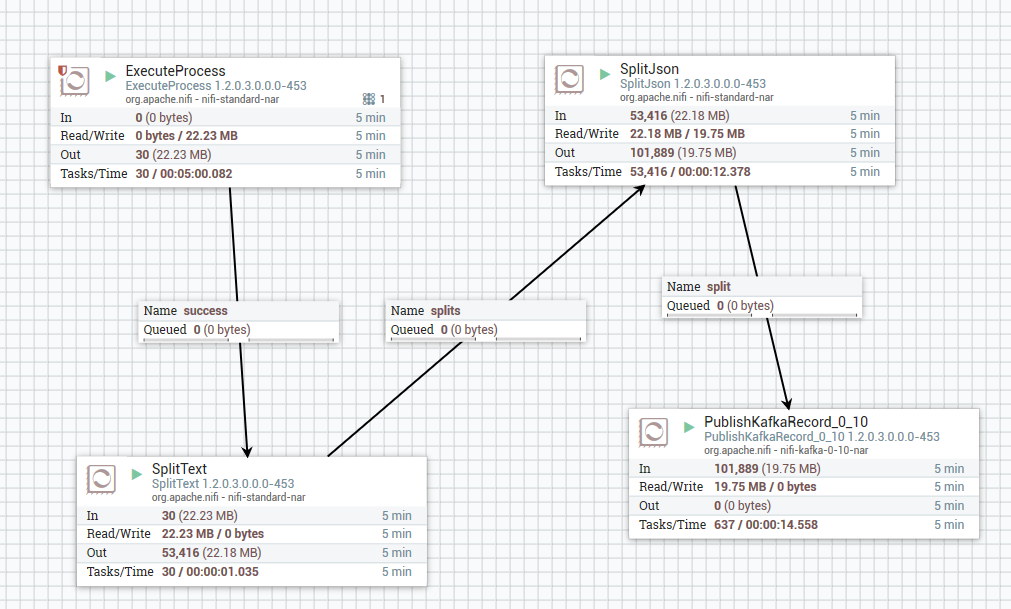
\includegraphics[width=0.7\linewidth]{Figures/nifipipeline}
    \caption{NiFi pipeline used for the ingestion from Satori}
    \label{fig:nifipipeline}
\end{figure}

In order to get into more details, let's list the entire pipeline:

\begin{enumerate}
    \item \textbf{ExecuteProcess} Processor, where the data fetching actually happens, it runs continuously the following script:
    
    \begin{code}
        \begin{minted}{Python}
with make_client(endpoint=endpoint, appkey=appkey) as client:
    
    class SubscriptionObserver(object):
        def on_subscription_data(self, data):
            for in_message in data['messages']:
                if all(len(str(x)) > 0 for x in in_message.values()):
                    fetched_data.append(json.dumps(in_message))
            got_message_event.set()
            
    subscription_observer = SubscriptionObserver()
    client.subscribe(
            "air-traffic",
            SubscriptionMode.SIMPLE,
            subscription_observer)
    
    while got_message_event.wait(10):
        if len(fetched_data) != 0:
            print(fetched_data)
     
        \end{minted}
    \end{code}
which basically uses Satori APIs to create a client subscribing to the Air Traffic JSON stream, fetching batches of JSON records, filtering those with empty values and printing each batch on standard output as a JSON array. ExecuteProcess will then create a \textbf{FlowFile} containing as a payload many JSON arrays from subsequent script calls, which will be the input for the following Processor;

\item \textbf{SplitText} simply deals with splitting a single FlowFile, with many JSON arrays, into that many FlowFiles containing only a single JSON array;
\item \textbf{SplitJson}, instead, deals with extracting all of the JSON Objects from the input JSON arrays, generating a FlowFile for each one of them;
\item \textbf{PublishKafkaRecord\_0\_10} is the NiFi Processor which publishes the incoming FlowFiles to a Kafka topic. Its required configuration needs the usual Kafka Producer settings: the broker list, a comma separated list of the broker listeners, in this case \texttt{master-1.localdomain:9092,master-2.localdomain:9092}, the topic in which each record needs to be published, \texttt{air\_traffic} and the security protocol used to publish, \texttt{PLAINTEXT}. Other than these settings, this Processor needs two components: a \textbf{Record Reader}, needed to deserialize the incoming FlowFiles, and a \textbf{Record Writer}, used to serialize each record before publishing it on Kafka. Said components are services provided by an \textbf{HortonworksSchemaRegistry}, a registry used to store Avro schemas\footnote{\textbf{\href{https://avro.apache.org/}{Avro}} is a data serialization system allowing to define types and possible values for JSON encoded records.} against which incoming records are validated to make sure they follow the specified schema. If validation succeeds, the record is then correctly published on the \texttt{air\_traffic} topic, serialized following the validated Avro schema.
\end{enumerate}

Data ingestion continues, then, in Kafka. As previously mentioned, a single topic called \texttt{air\_traffic} is used, configured with a retention time of 24 hours, a single partition, since throughput is approximately of $20000$ records per minute, accounting to 4 MB per minute, being a relatively sparse stream, and two replicas handled by both the active Kafka brokers.
\pagebreak

\subsection{Processing}

The main backbone of this use case is provided by Flink. After the data is being acquired from NiFi into Kafka, it's processed by a Flink application which then will persist enriched data on HDFS, MongoDB and Cassandra.
\\
Before talking about the Flink application per se, it's worth saying that Flink has been deployed on top of YARN with a Job Manager with 1GB of memory allocated and a single Task Manager with 3GB of memory and 3 slots for parallelism, for a total of 4GB and 4 vCPUs allocated on YARN. 

The Flink application has been written in Scala, making use of the appropriate Scala API provided by Flink. The job has been configured to checkpoint every minute, through an externalised checkpoint, to use as a state backend HDFS and use \texttt{EventTime} as the Stream Time Characteristic.

\subsubsection{Application}

\begin{figure}[h]
    \centering
    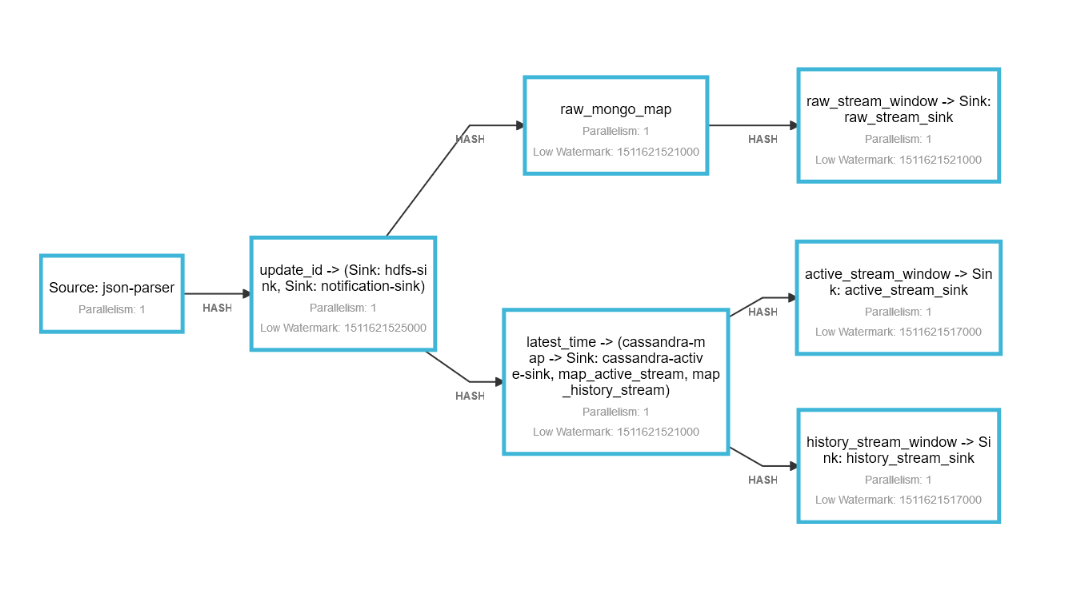
\includegraphics[width=0.8\linewidth]{Figures/flink_job}
    \caption{An overview of the complete DAG of the Flink application described in this section}
    \label{fig:flinkjob}
\end{figure}


\paragraph{Source}
The Flink application has a single source, a Kafka Consumer configured to consume from the \texttt{air\_traffic} topic connecting to both the active kafka brokers on \texttt{master-1} and \texttt{master-2}. Flink's built-in Kafka Consumer must be configured with a deserialization schema, which, in this case, parses from each JSON an \texttt{AirTrafficEvent} using Scala library \href{https://www.playframework.com/documentation/2.6.x/ScalaJson#The-Play-JSON-library}{Play-JSON}.
\\
\begin{code}
   \begin{minted}[breaklines]{Scala}
class JSONDeserializationSchema extends AbstractDeserializationSchema[AirTrafficEvent] {
       
    @throws[IOException]
    override def deserialize(message: Array[Byte]): AirTrafficEvent = {
       
    val obj = Json.parse(message)
    obj.as[AirTrafficEvent]
    }
       
    override def isEndOfStream(nextElement: AirTrafficEvent) = false
}
   \end{minted}
\end{code}

\texttt{AirTrafficEvent} is defined as a Scala case class with three fields wrapping all of the information contained in the original JSON: \texttt{FlightInfo}, containing flight, callsign, registration, origin, destination and aircraft, \texttt{InstantValues}, containing time, altitude, speed and course, and \texttt{Coordinates}, containing latitude and longitude.
\\
\begin{code}
    \begin{minted}[breaklines]{Scala}
//AirTrafficEvent definition
case class AirTrafficEvent
    (flightInfo: FlightInfo,
     coordinates: Coordinates,
     instantValues: InstantValues) extends Event(flightInfo, coordinates, instantValues) with Comparable[AirTrafficEvent]

//FlightInfo definition
case class FlightInfo
    (origin: String,
     destination: String,
     flight: String,
     aircraft: String,
     registration: String,
     callsign: String) extends Serializable

//InstantValues definition
case class InstantValues(speed: Int, altitude: Int, course: Int, time: Date) extends Serializable with Comparable[InstantValues]

//Coordinates definition
case class Coordinates(lat : Double, lon: Double) extends Serializable
    \end{minted}
\end{code}

Since Flink is using EventTime as Time Characteristic of the stream, a timestamp and a watermark should be assigned to every record, in order to be correctly managed for in order consuming and windows. The assigned timestamp and watermark are directly extracted using the \texttt{instantValues.time} field from the parsed \texttt{AirTrafficEvent}, via a \justify{\texttt{BoundedOutOfOrdernessTimestampExtractor}} to make sure that late events within 10 seconds are still correctly processed by Flink.

\paragraph{Operations}

Two main operations are performed on the data flowing through the DAG representing the application: the UID generation of the flight record currently processed and the event processing to get aircrafts which supposedly have arrived to destination.

UID generation is made through \texttt{UpdateIdFunction}, a stateful \texttt{ProcessFunction} processing each element of the stream according to the following pseudo-code:

\begin{minted}{Python}
if is_active_flight(element):
    id = old_id # mantained as state
else:
    id = id + 1
    notify_on_new_flight()
event = event_with_id(element, id)

return event
\end{minted}

It takes as input a \texttt{KeyedStream} of \texttt{AirTrafficEvent}s and outputs an \texttt{AirTrafficEventWithId} stream: the ID is an integer counter which gets increased each time a new instance of a flight is being detected and used to create the actual id of the outputted objects concatenating the flight id with this integer ID (e.g. the first instance of flight \texttt{AZ775} will have id \texttt{AZ775-1}). 

\begin{code}
    \begin{minted}{Scala}
    val streamWithId : DataStream[AirTrafficEventWithId]= stream
        .keyBy(_.flightInfo.flight)
        .process(new UpdateIdFunction())
    \end{minted}
\captionof{listing}{A KeyedStream of AirTrafficEvent processed into an AirTrafficEventWithId stream}
\end{code}
\pagebreak
The function handling the detection of a new instance of a flight is based off an heuristic strategy using the latest available information about the position, speed and time of the flight. This is needed because the stream may be inaccurate when it comes to transoceanic flights, passing over dead zones, without any radar at range being able to catch their transponder signals. The heuristic is described by the following Scala snippet:
\\
\begin{minted}[breaklines]{Scala}
val activeUpperBound = Time.minutes(5) // 5 minutes
val notActiveLowerBound = Time.hours(5) // 5 hours
val threshold = Time.minutes(120) // 60 minutes
val (last_lat,last_lon) = lastKnownPosition.value match {
    case null => return false
    case _ => lastKnownPosition.value
}
val last_speed = lastSpeed.value  match {
    case 0 => return false
    case _ => lastSpeed.value
}
val last_time = lastTime.value  match {
    case 0 => return false
    case _ => lastTime.value
}

if(new_time - last_time < activeUpperBound.toMilliseconds) true
else if(new_time - last_time > notActiveLowerBound.toMilliseconds) false
else
    Math.abs(distFrom(new_position, (last_lat, last_lon))/knotsToMetersSeconds(last_speed)
        - (new_time - last_time)/1000) < threshold.toMilliseconds/1000

\end{minted}

in which can be seen that there are three main conditions being checked:
\begin{enumerate}
    \item if the difference between the timestamps is less than a certain upper bound (default 5 minutes), meaning that we received an event from the current flight recently and implying the it is active.
    \item if the difference between the timestamps is greater than a certain lower bound (default 5 hours), meaning that we haven't received an event from the current flight in a while, implying it's a new instance of a flight. This case is used as a discriminant for flights flying over dead zones.
    \item provides a prediction based off the estimated time to reach the latest position from the previous last known position, at constant speed=last\_speed, and the actual time taken to reach the latest position.
\end{enumerate}

This way, we are able to be reasonably certain that an aircraft, even after passing over a dead zone for more than 5 minutes, is still flying towards its destination and we are not dealing with another instance of the same flight. A more accurate heuristic would be possible with a data source not cutting under 37000 feet and using an additional data source with the airports and their position, integrated within the stream structure.

Additionally, whenever a new instance of a flight is detected a side-output is used to forward outside of the \texttt{ProcessFunction} an \texttt{Alert} containing the relevant event, together with the event type, which is, in this case, \texttt{newAirplane}.
\\ \\
Just like it has been mentioned, the second operation executed on the stream concerns the event processing used to detect aircrafts arriving to their destination. Since it's been noted that the data stream is incomplete, in order to demonstrate \textbf{FlinkCEP} capabilities when it comes to event processing, instead of using a pattern that detects variations in altitude and speed to correctly determine the sequence of events implied by an aircraft approaching to an airport, it's been used a simple pattern based on the timing out of events sequences.

\pagebreak

The pattern is implemented as follows:
\\
\begin{minted}{Scala}
val airplaneArrivalPattern = 
Pattern
    .begin[AirTrafficEventWithId]("flying")
        .where(_.airTrafficEvent.instantValues.altitude >= 37000)
        .oneOrMore
    .notNext("disappearing")
        .where(_.airTrafficEvent.instantValues.altitude >= 37000)
        .within(Time.minutes(30))

// Associate KeyedStream with pattern to be detected
val patternStream  = CEP.pattern(streamById, airplaneArrivalPattern)
//Side output where timed out events are forwarded
val outputTag : OutputTag[Alert] = OutputTag[Alert]("side-output")
// How to handle timed out and in-time events
val result: DataStream[AirTrafficEventWithId] = 
    patternStream.select(outputTag) { //Timed out events
        (pattern: Map[String, Iterable[AirTrafficEventWithId]], 
        timestamp: Long) => {
            val alert = new Alert(pattern("flying").last, 
            AlertType.disappearedAirplane.id) alert
        }
    } { //In time events
        (pattern: Map[String, Iterable[AirTrafficEventWithId]]) =>
            pattern("flying").last}   
// Collect timed out events from the main stream
val alertStream = result.getSideOutput(outputTag)
alertStream.addSink(new NotificationSink()).uid("notification-sink")
    .name("notification-sink")
\end{minted}

and is basically structured on the analysis of a Keyed Stream, keying on the event id, such that if there's no event within 30 minutes from the last one, the pattern times out, an \texttt{Alert} is created, from the last event stored, and then forwarded to the notifications' sink.

\paragraph{Sinks}

The Flink application has three main sinks where data is forwarded to be stored after processing: \textbf{MongoDB}, \textbf{Hive via HDFS} and \textbf{Cassandra}. On these three sinks there are three types of data stores: a \textit{raw} data store where all the records are saved after being enriched with their unique ID, an \textit{history} data store where it is saved a single record per flight, updated as needed, and an \textit{active} data store used for live monitoring purposes. An additional sink is used for the \texttt{Alert}s constructed during the stream processing.

\textbf{MongoDB} is used as sink for all of the three data stores, with adequately defined collections, while \textbf{Cassandra} is used for the \textit{active} data store, and \textbf{Hive} via HDFS is used only for the \textit{raw} and \textit{history} ones.

\pagebreak

Cassandra Sink in Flink is added through the \texttt{CassandraSinkBuilder} used to specify the query to be used while inserting the records in the table:
\\
\begin{minted}{Scala}
// Add sink to Cassandra cluster
CassandraSink.addSink(
    airtrafficEvents
        .map(_.toCassandraTuple)
        .javaStream)
.setQuery(
    s"""UPDATE air_traffic.active
    |SET lat = ?, lon = ?, speed = ?,
    |    altitude = ?, course = ?, flight = ?,
    |    origin = ?, destination = ?, aircraft = ?, time = ?
    |    WHERE id = ?;""".stripMargin)
.setClusterBuilder( new ClusterBuilder {
def buildCluster(builder: Cluster.Builder): Cluster = {   
    builder.addContactPoint("slave-1")
    builder.addContactPoint("slave-2")
    builder.addContactPoint("slave-3")
    builder.addContactPoint("slave-4")
    builder.build()
}
}).build()
\end{minted}

\pagebreak

On Cassandra's cluster, composed as already mentioned previously, by the four slave nodes, has been specified an \texttt{air\_traffic} keyspace, configured with a replication factor of 3 via the replication strategy \texttt{SimpleStrategy}. Within this keyspace the following table has been defined:
\\
\begin{minted}{SQL}
CREATE TABLE air_traffic.active (
    id text PRIMARY KEY,
    altitude int,
    course int,
    destination text,
    flight text,
    aircraft text,
    lat double,
    lon double,
    origin text,
    speed int,
    time timestamp
) WITH default_time_to_live = 600
       AND gc_grace_seconds = 3600
\end{minted}

in order to contain all of the active aircrafts currently flying. All of the default configurations have been maintained, except for the TTL of the records which has been configured to 10 minutes and the interval of the garbage collection of the table tombstones (expired records after the TTL) which has been set to 1 hour, instead of 1 day.
\\ \\
Notifications sinks are rather simple \texttt{SinkFunction}s which take as input the \texttt{Alert} and make an async \texttt{POST} request, through a \href{https://dispatchhttp.org/Dispatch.html}{Dispatch} asynchronous HTTP client, to the local notification server, implemented using Firebase FCM, about which we'll talk about later on.

\pagebreak
Hive is not the direct destination of the Flink sink. As a matter of fact, an HDFS sink is used to write all of the records in JSON format, partitioned in folders according to their timestamp. As a result, each event will be bucketed in the appropriate folder and this folder will be considered as a partition of an Hive external table configured using the \textbf{JsonSerDe} to read all of the files.
\\
\begin{minted}{Scala}
val hdfsSink = new BucketingSink[AirTrafficEventWithId](hdfs_path)
hdfsSink.setBucketer(new EventDateTimeBucketer("YYYY-MM-dd"))
hdfsSink.setBatchSize(1024 * 1024 * 64) // 64MB files size

streamWithId.addSink(hdfsSink).uid("hdfs-sink").name("hdfs-sink")
\end{minted}

\pagebreak
while the Hive external table is defined as it follows:
\\
\begin{minted}[breaklines]{SQL}
CREATE EXTERNAL TABLE IF NOT EXISTS json_dump
( `origin` string,
`flight` string,
`course` int,
`aircraft` string,
`callsign` string,
`registration` string,
`lat` double,
`lon` double,
`altitude` int,
`speed` int,
`destination` string,
`time` timestamp,
`_id` string)
PARTITIONED BY (`dt` string)
ROW FORMAT SERDE 'org.apache.hive.hcatalog.data.JsonSerDe'
WITH SERDEPROPERTIES ('timestamp.formats'='YYYY-MM-dd HH:mm:ss.SSS')
STORED AS TEXTFILE
LOCATION '/flink/air_traffic/json_dump';
\end{minted}

Starting from this very table, which maintains records in text format, uncompressed, further optimizations will be performed before the final storage within Hive.

\subsubsection{Post-processing: HDFS to Hive}

As we already determined, Hive is not the direct target of Flink, since we're using an Hive external table to read all of the Json files written by the HDFS sink. Using a textfile format is not optimal for storage purposes, since it's not a compressed format and we'd like to save as much storage as possible. For this reason an additional table, in the appropriate database in Hive, has been defined to be the final target of the raw stream written in HDFS. Additionally, from this table, another table called history is filled, aggregating all of the records of a flight in a single record with arrival date and departure date.

To sum up, there are three tables stored in Hive:
\begin{itemize}
    \item \texttt{json\_dump}, external table reading the Json files written by Flink;
    \item \texttt{raw} in \texttt{air\_traffic} database, containing an optimized version, for storage and query purposes, of \texttt{json\_dump} 
    \item \texttt{history} in \texttt{air\_traffic} database, aggregating \texttt{raw} creating a single record for each flight.
\end{itemize}

\pagebreak

The raw table is defined to use ORC as storage format, to use Hive partitioning on the date and to be clustered in 100 buckets, in order to make sure that, if needed, a query concerning a certain subset of flights wouldn't read all of the files composing the table.
\\
\begin{minted}[breaklines]{SQL}
CREATE TABLE IF NOT EXISTS air_traffic.raw(
`origin` string,
`flight` string,
`course` int,
`aircraft` string,
`callsign` string,
`registration` string,
`lat` double,
`lon` double,
`altitude` int,
`speed` int,
`destination` string,
`time` timestamp,
`_id` string)
PARTITIONED BY (`dt` string)
CLUSTERED BY (flight) INTO 100 BUCKETS
STORED AS ORC;
ALTER TABLE air_traffic.history SET SERDEPROPERTIES("timestamp.formats"="YYYY-MM-dd HH:mm:ss.SSS");
\end{minted}

\pagebreak

The history table is instead defined with the additional fields \texttt{arrival\_date} and \texttt{departure\_date}, removing all of the instant values, deemed as not needed, as it follows:
\\
\begin{minted}{SQL}
CREATE TABLE `history`(
`_id` string, 
`date_depart` timestamp, 
`date_arrival` timestamp, 
`flight` string, 
`callsign` string, 
`registration` string, 
`aircraft` string, 
`origin` string, 
`destination` string)
PARTITIONED BY (`dt` string)
\end{minted}

\pagebreak

Both these tables are filled in a periodic batch operation, scheduled every 20 minutes, through \texttt{INSERT OVERWRITE} queries on the current partition (date): whereas the \texttt{raw} is a simple overwrite from \texttt{json\_dump} as they have the same schema,  \texttt{history} aggregates the time field via \texttt{MAX()} and \texttt{MIN()} Hive aggregated functions as shown below:
\\
\begin{minted}{SQL}
INSERT OVERWRITE TABLE air_traffic.history 
PARTITION(dt="${PARTITION}")
(SELECT
    `_id`,
    MIN(time) AS date_depart,
    MAX(time) AS date_arrival,
    flight,
    callsign,
    registration,
    aircraft,
    origin,
    destination
FROM air_traffic.raw
WHERE dt="${PARTITION}"
GROUP BY 
    `_id`,
    flight,
    callsign,
    registration,
    aircraft,
    origin,
    destination)
\end{minted}

Periodic scheduling has been set using \texttt{crontab} functionalities of CentOS, which is used to execute a Python script called \texttt{hive\_loader} which executes the needed queries. \texttt{Hive\_loader} has four flags used to determine which queries has to be executed:
\begin{enumerate}
    \item \texttt{bootstrap}, which creates all of the tables used.
    \item \texttt{update}, which controls the scheduled execution for the update of raw and history tables.
    \item \texttt{add\_partition\_update}, used after midnight to definitively update \texttt{raw} and \texttt{history} of the previous day, while adding a new partition to \texttt{json\_dump}.
    \item \texttt{drop\_partition}, used to drop the previous day partition, before deleting it.
\end{enumerate}

Together with the aforementioned tables, additional tables have been created and filled to be available to Tableau for visualisation purposes:

\begin{itemize}
    \item \texttt{aircrafts}, containing the ID model and its capacity in terms of number of passengers.
    \item \texttt{airports}, containing, for each airport, its complete name, its IATA code, its continent and its ISO country and region codes.
\end{itemize}

\subsection{Serving \& Security}
Our infrastructure's security is handled on several layers by a variety of services striving to offer access on data and visualisations to the users and to let the developers maintain and upgrade the system while providing extensive security on the data and protection from unauthorized access.

\begin{figure}[h]
	\centering
	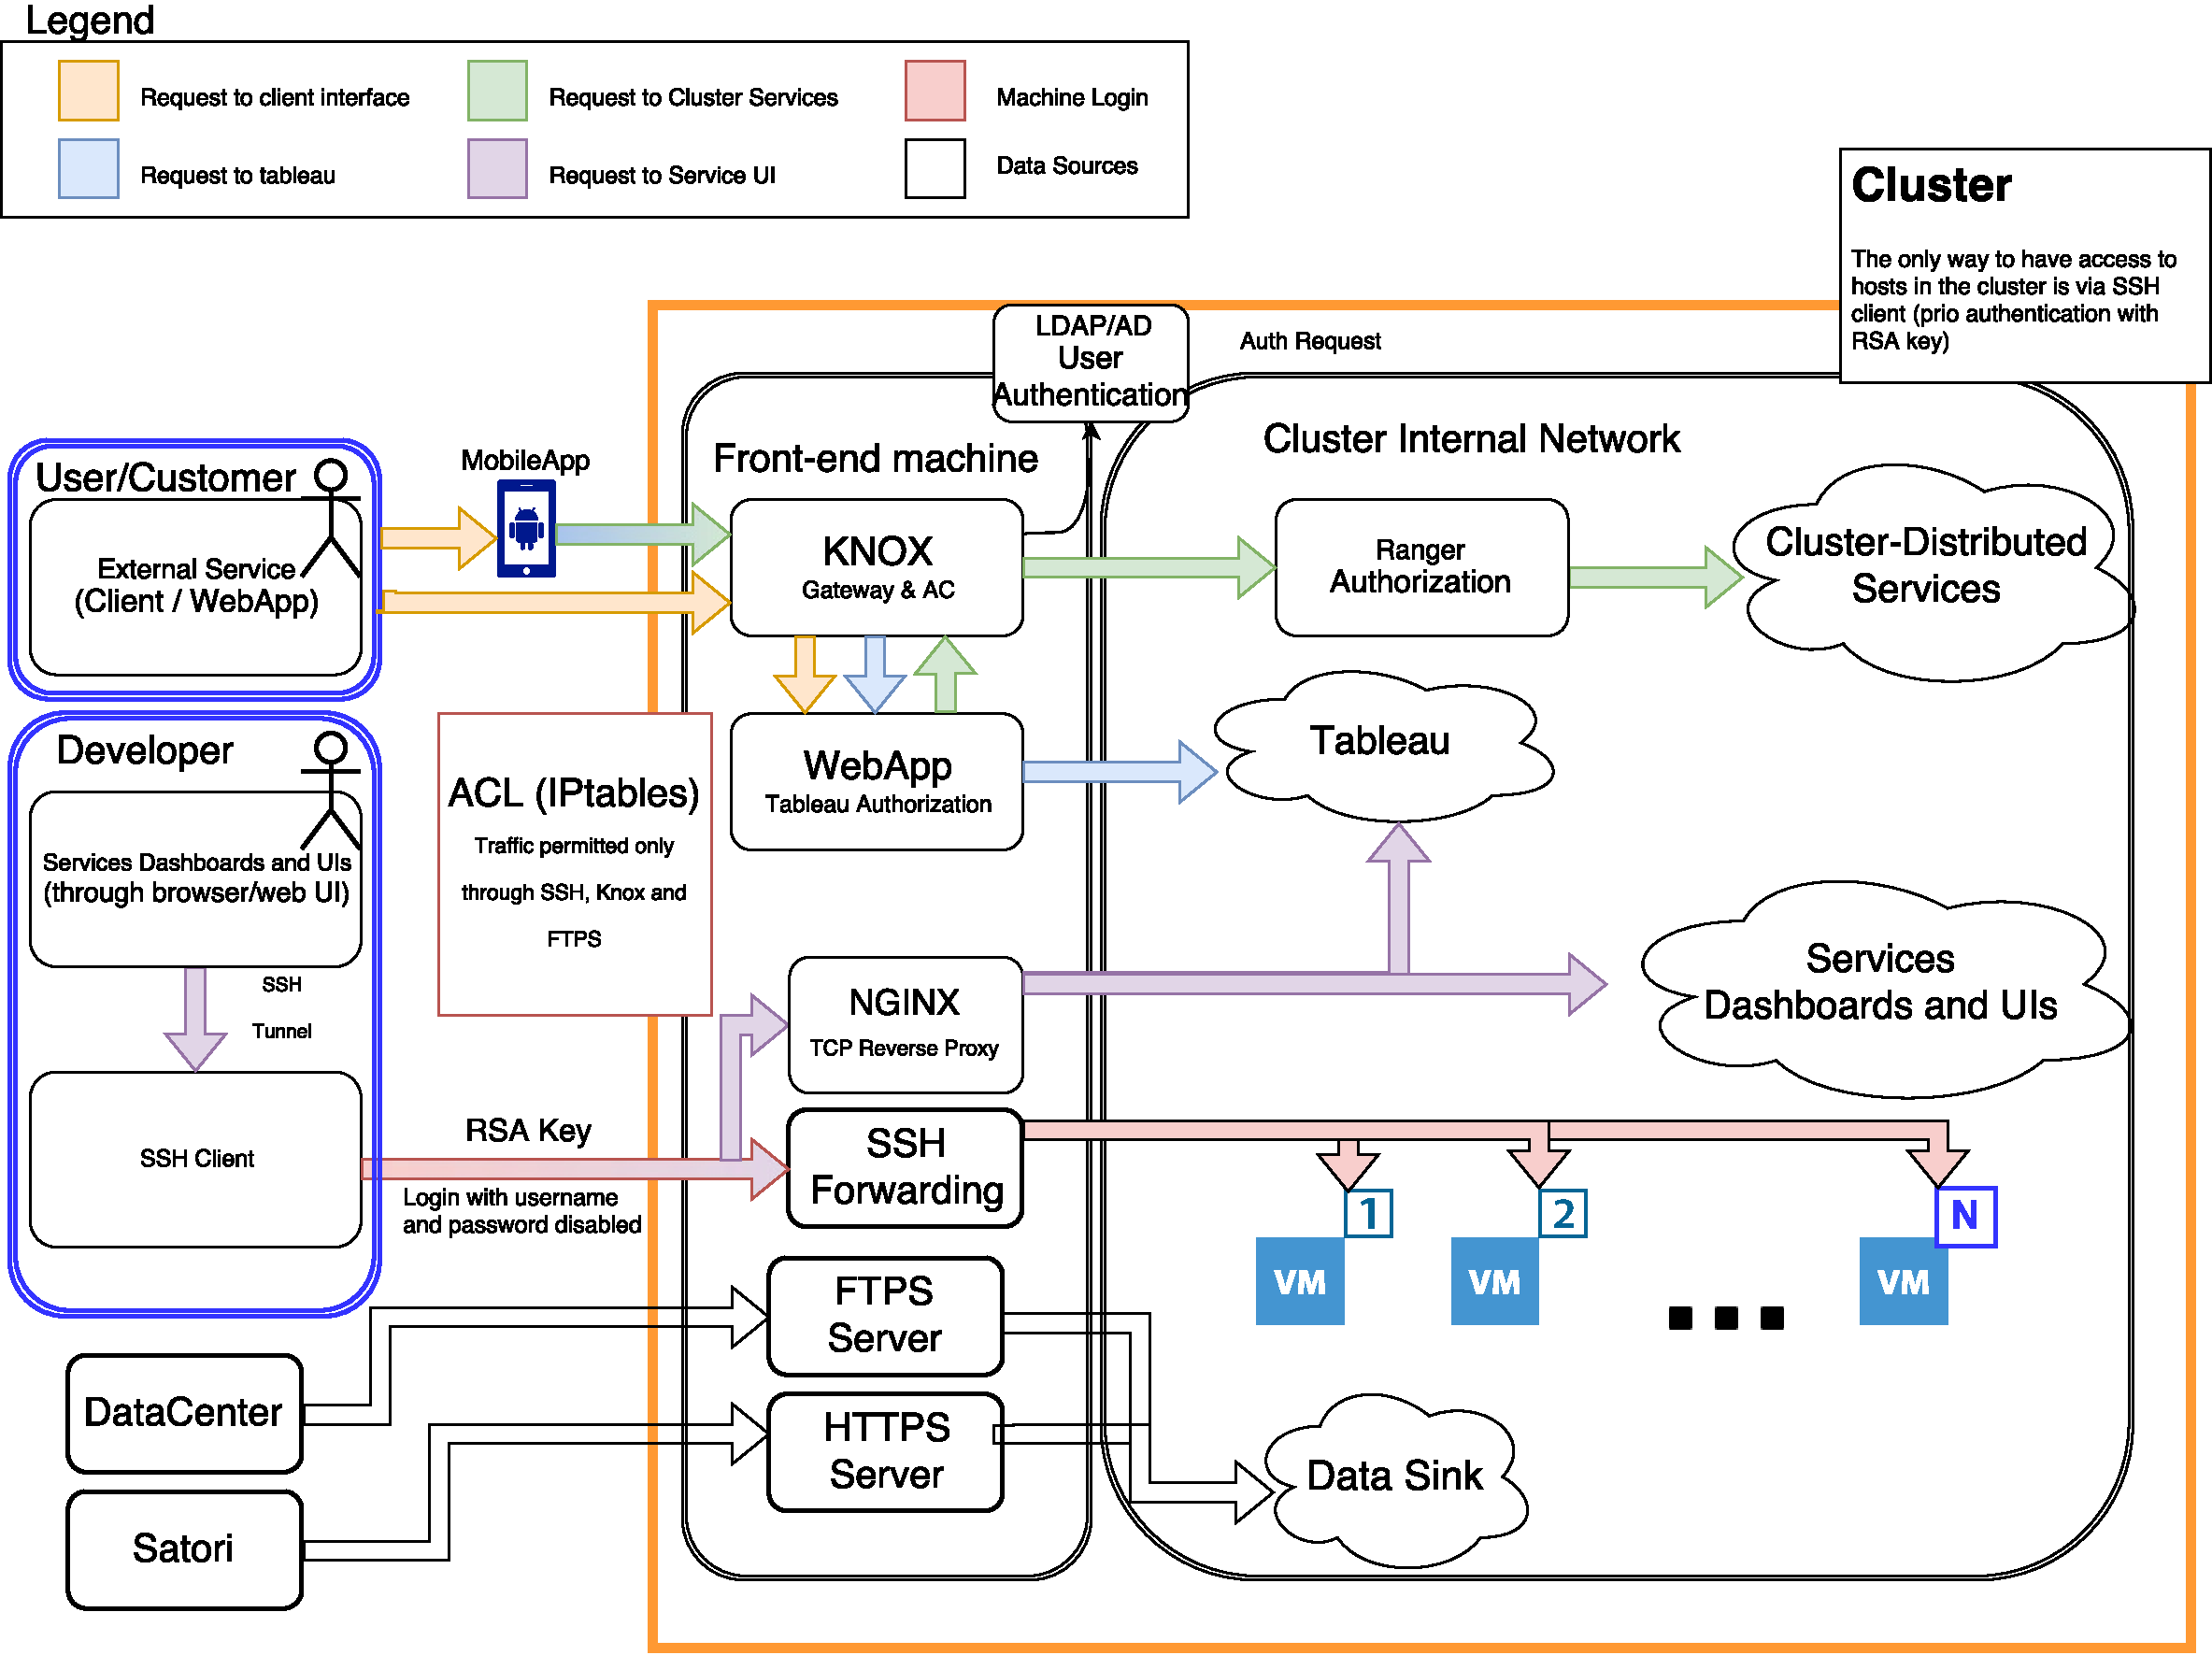
\includegraphics[scale=0.4]{Figures/SecurityStructureDiagram}
	\decoRule
	\caption[Security Structure Diagram]{A diagram to represent our Security Structure}
	\label{fig:SecurityStructureDiagram}
\end{figure}

We have structured the Security and Serving architecture through two main abstractions: the \textbf{cluster} and the \textbf{flows}.
\subsubsection{Cluster}
The \textbf{cluster} is our whole Big Data Infrastructure comprised of several nodes which for our purposes are divided as such:
\begin{itemize}
	\item One (or two in High Availability) Domain Controller, which handles user creation, update and authentication.
	\item One (or two in High Availability) Front End node, which manages access to the cluster's services and data.
	\item Several Inner Cluster nodes, the machines on which visualising, processing and storing is actually done.
\end{itemize}

\paragraph{Domain Controller}
The Domain Controller is not accessible from outside the cluster and can communicate freely with the Front End and the Inner Cluster Nodes.\\
It hosts Active Directory, a directory service by Microsoft comprised of several components for domain and security management such as LDAP, Kerberos, and DNS.\\ \\
As a directory service, the Active Directory instance consists of a database containing an hierarchy of objects, objects are a very high abstraction that can represent a variety of things, but for our purposes can either be Users or Groups; Groups contain one or more Users and Users may be part of one or more Groups. \\Users are identified by a username and a strong password, thus the Domain Controller can authenticate an Agent thanks to this information. \\
Through LDAP, authorized Users can access and modify Objects in the Active Directory. Each authentication, whether failed or successful is logged.\\ \\
We have defined two groups: \texttt{cluster\_users} and \texttt{cluster\_operators}, the meaning of which is further specified down the line by each layer of protection.

\paragraph{Front End}
The Front End node is the only machine accessible from outside the cluster and can communicate with the Domain Controller and the Inner Cluster nodes. \\
Access to the Front End from outside is possible through a selected number of ports and only with secure protocols (HTTPS, FTPS and SSH), this is obtained with the use of ACLs, implemented on CentOS through iptables. The Front End features Apache Knox and Nginx to route requests to the right services and stores RSA private keys of all the Inner Cluster nodes plus a public one for each developer's own private key, so that passwordless SSH connections can be established from developers' machines to Front End and from Front End to Inner Cluster nodes. \\
\\
Nginx is a HTTP and HTTPS reverse proxy that also supports TCP reverse proxying and can be used to route whatever HTTP request or TCP connection from the Front End machine to the proper Inner Cluster node's service. \\
\\
Apache Knox also serves as a reverse proxy, this time specifically for Hadoop cluster's services requiring authentication and authorization. Its topology is implemented so that an authorised Active Directory user called Knox.domain through LDAP can ask for authentication on an incoming request's sender and access to lists of Users and Groups.\\ If the user is authenticated, Knox can then grant access to the request, thanks to the information on Users and Groups, to the target service and route it accordingly or deny it. \\ Outcoming requests are bundled with the authenticated username, so that inside the Inner Cluster nodes other services can use that information securely. Requests at this stage are logged both denied and accepted with the name of the alleged requester to be investigated in case of failures or attempted breaches.\\ \\
The topology is set so that all our custom services for access to MongoDB and Hive are available to all users belonging to the cluster\_users or cluster\_operators group, while the standard Hadoop services are available only to those in the latter.
\\
\\
The Front End machine also hosts programs for data ingestion, an FTPS server and a NodeJS application that serves the WebApp.

\paragraph{Inner Cluster Nodes}
All the other nodes in the Cluster are considered Inner nodes as they are barred from outside and can only communicate with the Domain Controller and the Front End. \\
These machines hold all processing services, databases and visualisation tools plus the interfaces to access their resources. Here requests incoming from the Front End have been already authenticated and given access, but each service can enact additional policies on those to add a layer of security and to protect from mistakes (i.e. DROP DATABASE). \\ \\
While each service might manage its own policies, most Hadoop applications delegate this burden to Apache Ranger: Ranger, thanks to its Usersync agent synchronises its list of Users and Groups with the Active Directory's one, so that further authorisation policies can be defined on the same cluster\_users and cluster\_operators seen before. \\ \\
 Thus we have decided to give users in cluster\_users clearance for the use of SELECT on our Air-Traffic database, while deletions are forbidden to them, on the other end users in cluster\_operators are also able to update and delete records.
\\ At this level requests are logged again, to log failed authorisations and to assign actions' responsibilities to the appropriate users.

\subsubsection{Flow}
We define the flow, in the context of the security of our system, as the path requests and responses travel from a class of external Actors to the cluster and back.
\\ \\
In general the flow starts from an Actor outside the cluster sending a request (i.e. A User through a MobileApp), the request is received by the Front End Node, accepted or denied; accepted requests are then forwarded and routed to the target Inner Node's service which handles the request and generates a response accordingly, the response is then set back following the same path backwards to the Actor.
\\ \\
We have distinguished three different flows each pertaining to a different Actor:
\paragraph{User}
A user, which is a person or agent requesting access to our stored data, can query our databases and view visualisations built upon stored data service through a WebApp or a Mobile App.\\
Queries are sent to our custom REST APIs to Knox on the Front End machine; the user, who must be present in Active Directory and be part of cluster\_users, is authenticated and authorised to proceed with its request, this request now routed to the Inner Cluster is received by our REST servers, parsed into queries and sent to the appropriate database with the user's credentials, the query is received by MongoDB security or Apache Ranger for Hive, whatever the recipient its policies are enforced on the request; the result of the query is then sent back to the REST server which encapsulate it and send it back as a response to the user.
\\ \\
Visualisations are requested to the WebApp from outside the cluster, the WebApp requires a login for authentication an then authorises the user following its own policies as a Tableau user or operator, the WebApp then requests tokens to be consumed watching visualisations on behalf of the user and then responds with a HTML page embedding the visualisations and tokens. This method prevents the need of having to authenticate the same users multiple times.
\paragraph{Developer}
While able to access the cluster as clients, the developers can also connect to the Front End through a SSH client provided they have the Front End private key as username and password are disabled, while connected they can further their connections to all nodes to access the local file system. What's more, through tunnelling several TCP connections can be forwarded through the SSH connection from the developer localhost to the Front End machine; there Nginx routes Front End local connections to several clusters' machines, providing a safe passage from the developer's machine to the required Dashboard or User Interface.
\paragraph{Data Source}
Lastly Data Sources must be able to send data to our secured clusters to be stored on the databases, in order to do that two options are available: an application on the Front End can pull data constantly on an endpoint (for example through HTTPS) or the providers can push data on a server on the Front End (for example through FTPS), then another application is responsible to transfer newly acquired data from the Front End to the Inner Cluster Nodes

\subsection{Accessory Services}

While not strictly related to Big Data, the results we archive and process may be used for several different endeavours; we wanted to add an additional feature for presentation, other than the aforementioned REST APIs and Visualisations, targeted for mobile devices in the form of push notifications.
\\ \\
To show the capabilities of this system, we have decided to send Push Notifications whenever a plane departs and is directed towards one of our airports of interest or whenever a plane is approaching its destination, descending below 37000 feet of altitude.
\\ \\
To offer this service we have implemented a solution based on one of the many components of the Google Mobile Platform: Firebase Notifications.

\subsubsection{Firebase Notifications}

Firebase Notifications is a service for mobile and browser push notifications offered through a REST API listening on Google Firebase servers; the requests sent to this API are formatted in JSON specifying information on the message sent and on the receivers.
What's more, the Firebase Server assigns to each device attached to our application a unique and expiring token to identify what devices will be receiving each notification.
\\
In more detail, Firebase Notifications supports two different ways to send messages.

\begin{itemize}
	\item \textbf{Token based messaging}: The request for the notification includes a list of the tokens assigned to the recipient devices. 
	\item \textbf{Topic based messaging}: The devices are required to subscribe to topics, requests are sent specifying the topic of which the notification is part of, so that subscribers can receive it.
\end{itemize}  

Seen that our topic in this case would have been airports, whose list is giant and ever growing, we have concluded that topic based messaging would be highly impractical and therefore chosen to use the token based solution and to handle the routing of notifications through a filtering application.

\subsubsection{Local Server}
To handle users' data, filtering of notifications and the construction of requests to be forwarded to Firebase, we have implemented a middleware server in JavaScript, listening on internal nodes, which offers a REST API customised for our needs.
\\
The server manages users' data, keeping a table on Hive representing the connection between Device Unique ID, Notifire Token and a list of airports the user is subscribed to. Changes to this table can be issued by the users through a request to the server, it is mandatory for the mobile application to send an update after obtaining a new token from Firebase, so that the table is always up to date.
The table is also cached in memory for performance's reasons.
\\ \\
As mentioned the server offers a REST service to ingest notifications and forward it to Firebase. In more detail, the server expects a JSON containing information on a departing plane such as: airport of origin, airport of destination, type of aircraft, flight number and other spatial or temporal values.
\\ \\
For each received and accepted JSON, the server writes a list of tokens that are subscribed to the airport of destination and creates a message informing of the departure. It then creates a request with those data and send it to the Firebase server which in turn sends the actual notification to all target devices and responds back to our server with a report of the action.


\subsection{Visualisation}

With the files processed by Flink and stored on MongoDB, Hive and Cassandra we have built several workbooks on Tableau:

\begin{itemize}
	\item \textbf{Live Map}: A map of the world tracking all active flights in real time (Using either MongoDB or Cassandra as data source).
	\item \textbf{Inbound Flow}: Set of different charts to analyse the flow of flights directed towards an airport of choice (Using either MongoDB or Hive as data source).
	\item \textbf{Outbound Flow}: Set of different charts to analyse the flow of flights departing from an airport of choice (Using either MongoDB or Hive as data source).
	\item \textbf{Flight Route}: A route tracked on the map of the world showing the path followed by an aeroplane of choice (Using MongoDB as data source).
\end{itemize}
\subsubsection{Connection to Data Source}

In order to connect Tableau to a data source two middlewares are required: a \textbf{Connector}, to translate Tableau's own VizQL to the target database query language, and an \textbf{ODBC} in which to specify the address and port in which the database is to be found to do the actual connection.
\\
Tableau uses internally a relational model and VizQL is therefore a query language for such models; while for relational databases, such as Hive, the query translation is pretty straightforward, for NoSQL databases like MongoDB and Cassandra the conversion is done with an additional step in which a schema is produced to translate the Document based and Key/Value models into relational models.

\subsubsection{Live Map}
The live map is used to monitor and track in real time planes flying all over the world. Data for this view are collected from Cassandra's Active table or MongoDB's Active collection through a live connection; this connection allows us to refresh the map as soon as new data are available in the database.
\\
The two most important variables for the construction of such graphic are latitude and longitude, used by Tableau to draw a marker on the map. Such marker, by default, is a bullet point, but in order to add a new dimension to the view we added a custom marker showing a plane directed towards the actual direction the flight is headed to.
\\
As for interactivity from the view, it is possible to read other details of a single plane or to use one or more of several filters:
\begin{itemize}
	\item \textbf{Origin}: Airport whence the plane departed.
	\item \textbf{Destination}: Airport where the plane is headed towards.
	\item \textbf{Flight}: The unique code given to a flight.
	\item \textbf{Aircraft}: The aircraft's model's unique code.
\end{itemize}

Figure \ref{fig:LiveMap} shows a close up of the middle east without any filtering.
\begin{figure}[h]
	\centering
	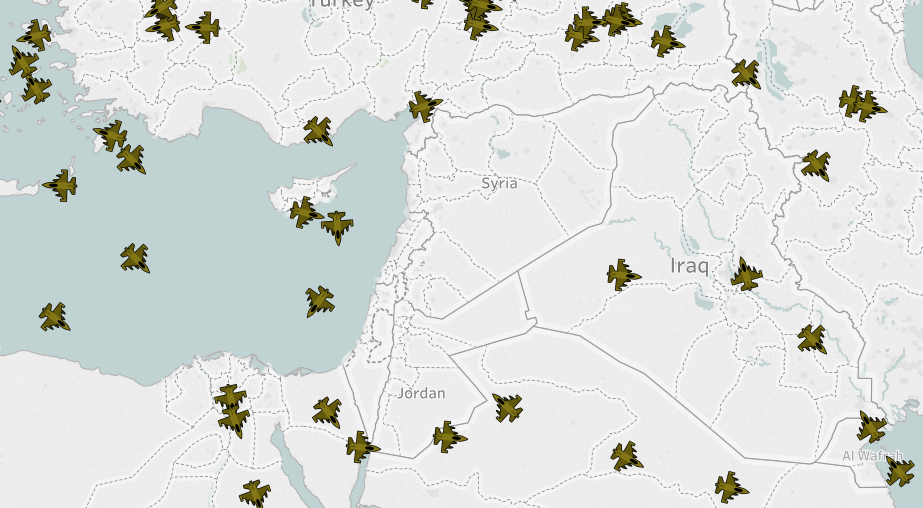
\includegraphics[width=0.9\linewidth]{Figures/LiveMap.png}
	\caption{A close up of the live map over the middle east}
	\label{fig:LiveMap}
\end{figure}

\subsubsection{Inbound Flow}

The second view built aims to present historical data of flights that have landed at an airport. For this kind of periodic analysis for which we have not need of real time connections, we have chosen to use the extract connection; this extract is updated each day and guarantees superior performances in charts' rendering.
\\
Before the extraction, we have set up a join between historical data and collections with information on aircrafts and airports in order to enrich the data source, furthermore fields not utilised in the presentation have been cleansed to lighten the load.
\\
Data are presented in three dashboards focusing on:

\begin{itemize}
	\item \textbf{Flights}: The total number of flights landed at an airport.
	\item \textbf{Aircraft}: The type of aircraft of those flights.
	\item \textbf{Passengers}: The total number of passengers landed at an airport.
\end{itemize}

Whatever the focus, the first useful operation is to filter by selecting an airport for which to analyse the flow. After that several temporal filters are available with complete control of the granularity of time through drill-down and drill-up. It is also possible to change type of chart from classical histogram to geographical maps and heat maps.

Figure \ref{fig:FlightsViz} shows a histogram depicting the flow of flights from the world towards Albuquerque in the month of November from 8 AM to 8 PM, day by day.

\begin{figure}[h]
	\centering
	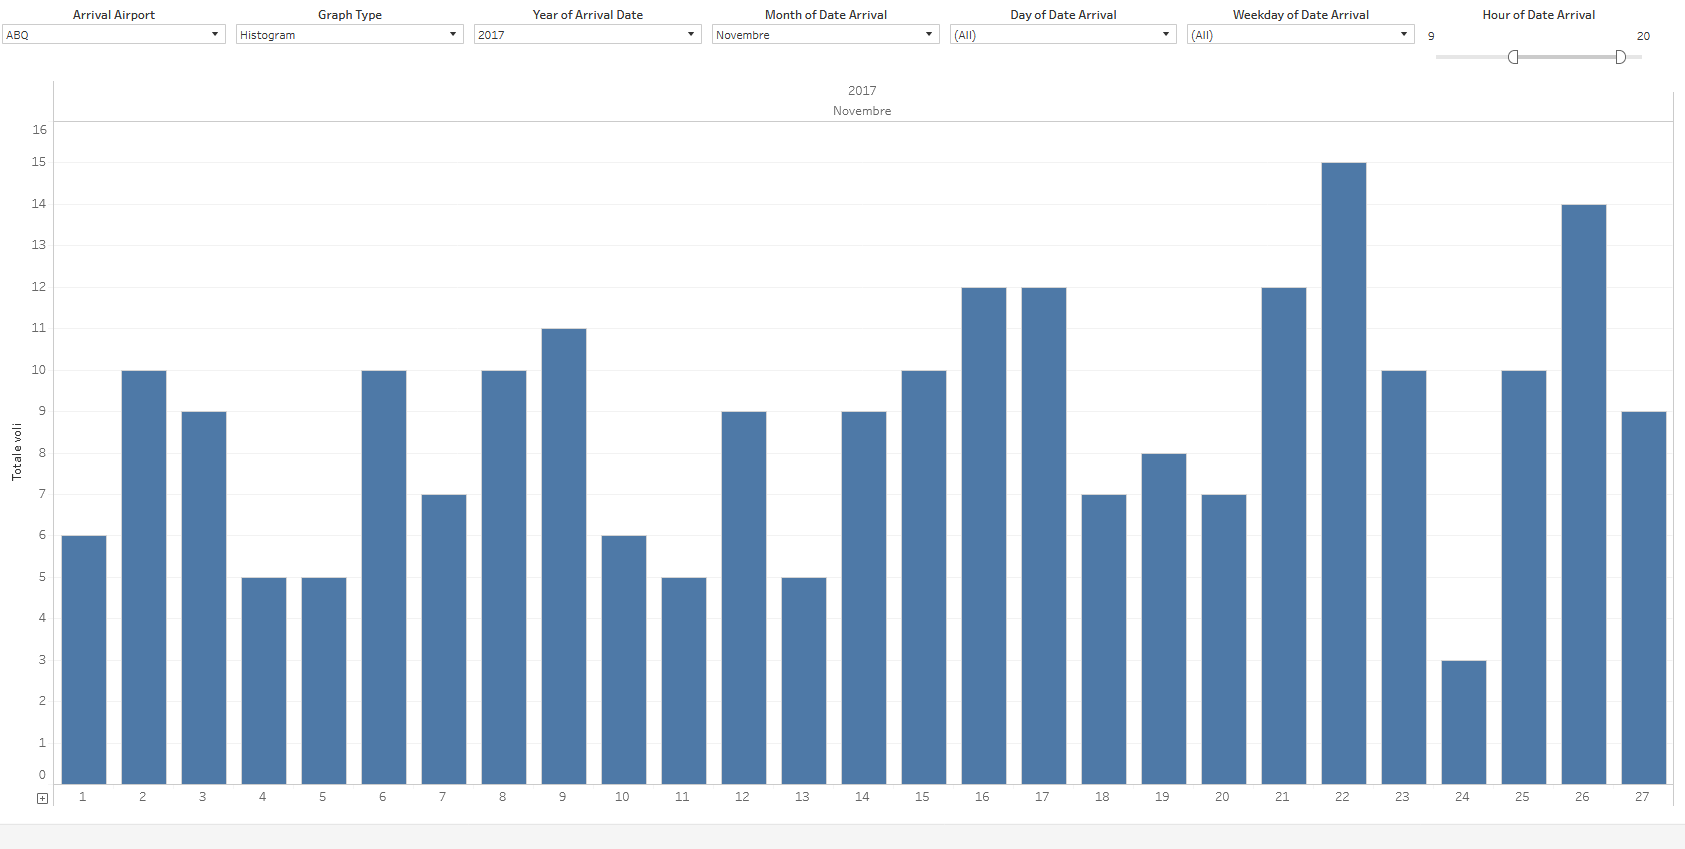
\includegraphics[width=0.9\linewidth]{Figures/FlightsViz.png}
	\caption{Inbound Flow for Albuquerque day by day 8 AM to 8 PM, November}
	\label{fig:FlightsViz}
\end{figure}

\subsubsection{Outbound Flow}
A carbon copy of the inbound flow has been realised to analyse the flow departing from an airport.\\
This duplication is done in order to optimise performances on both views. From an implementation point of view the only change is in the join condition to use during the extract creation and the use of the time of departure as timestamp, instead of the time of arrival.

Figure \ref{fig:PassengersViz} shows a map depicting the main destinations of the passengers departing from Genoa in October and November.

\begin{figure}[h]
	\centering
	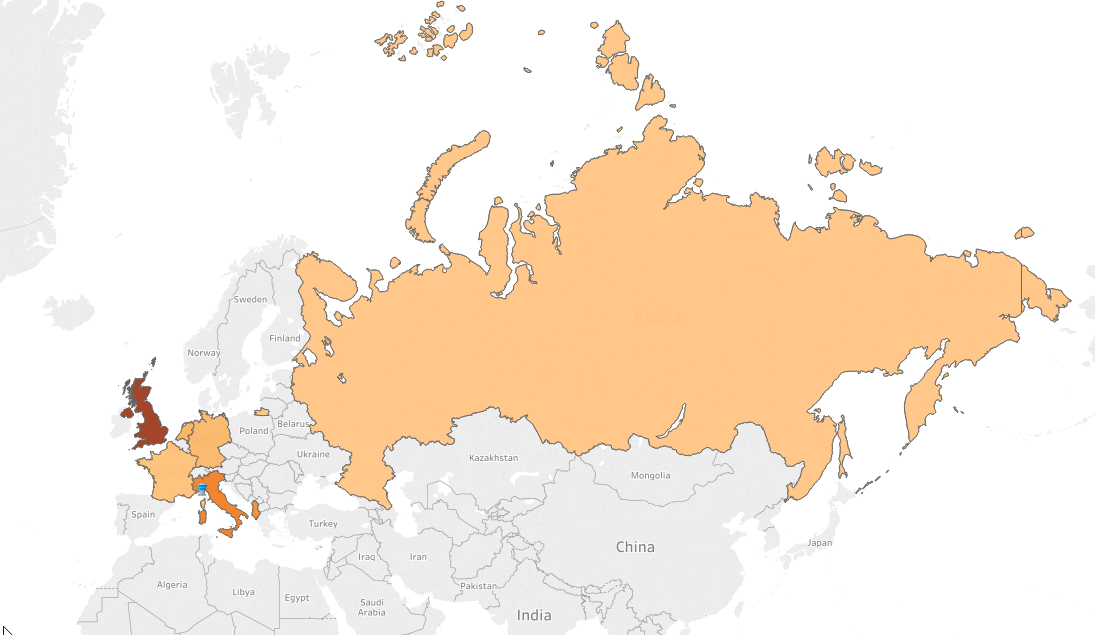
\includegraphics[width=0.9\linewidth]{Figures/PassengersViz.png}
	\caption{Outbound Flow of passengers for Genoa, October and November}
	\label{fig:PassengersViz}
\end{figure}

\subsubsection{Flight Route}
Given a flight code, it is possible to draw the path the aeroplane followed on each day for that route. This view shows the limits of Satori as an end-point, because we can only see messages coming from a height over 37000 feet, cutting the taking off and the landing parts of the fare.

 Figure \ref{fig:RouteViz} shows, through a set of points coming from consequent messages from the same plane, the route of flight UA914, from Paris to Washington, of October 25th; here it can be seen the filter cutting data below 37000 feet in action.
\begin{figure}[h]
	\centering
	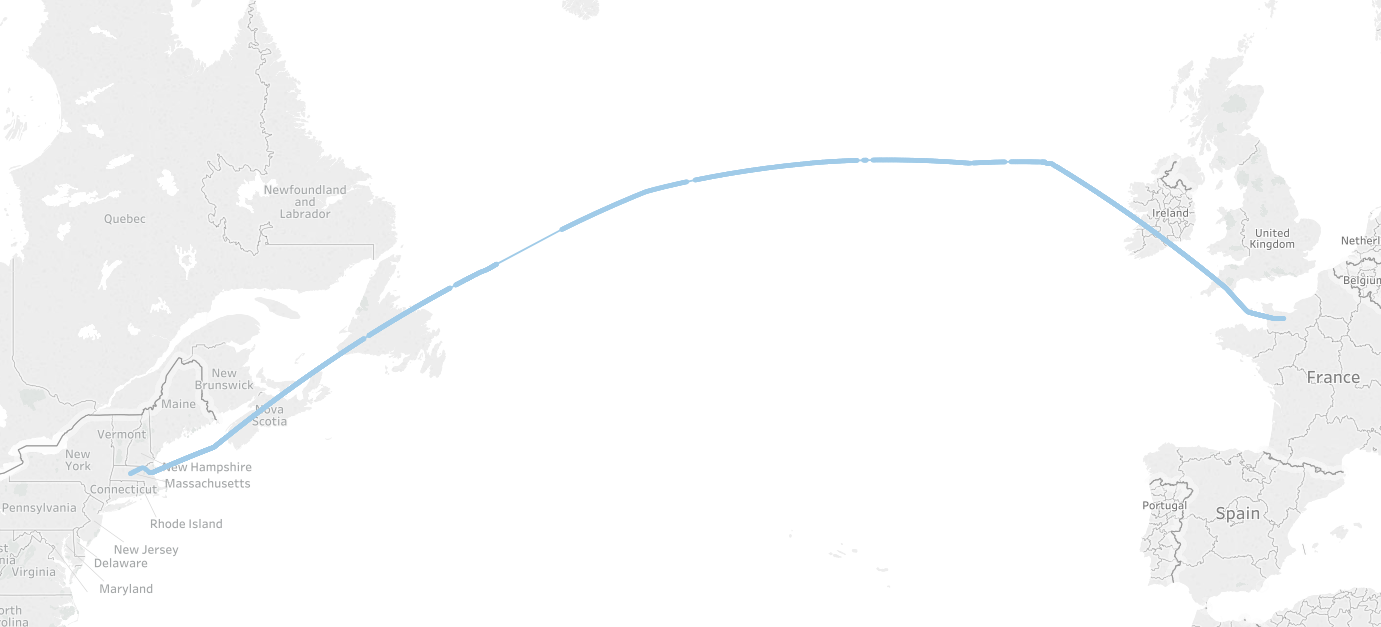
\includegraphics[width=0.9\linewidth]{Figures/RouteViz.png}
	\caption{The route of flight UA914, from Paris to Washington, of October 25th}
	\label{fig:RouteViz}
\end{figure}
This view is built with a live connection with the use of Custom SQL. Thanks to the definition of an ad hoc query, MongoDB's Raw collection is queried using the flight code as a parameter.
The query is then converted to an aggregation pipeline in MongoDB with a dedicated process, resulting in a response within few seconds, in spite of the huge size of the collection (more than a billion documents).
\subsubsection{Publishing on Tableau Server}
Once the workbooks have been created, we proceeded by publishing all the views on Tableau Server. For this purpose, we have defined two user groups with different rights: the Devs who inherit the powers and rights of the Publisher and can create, edit and interact with the workbooks; the Users which inherit the right of the Interactor and can, therefore, only interact with the workbooks.

In order to use the views freely, it had been necessary to save the required credentials for the authentication on the data sources directly on the Tableau workbook.
Finally, we have scheduled a daily update at 4 AM to refresh the extracts for the visualisations of historical data.